\documentclass[journal]{IEEEtran}

\usepackage[T1]{fontenc}
\usepackage{amsmath,amssymb,amsthm}
\usepackage{booktabs}
\usepackage{array}
\newcolumntype{L}[1]{>{\raggedright\arraybackslash}p{#1}}
\usepackage{cite}
\usepackage{graphicx}
\usepackage{multirow}
\usepackage{xcolor}
\usepackage{url}
\usepackage{tikz}
\usetikzlibrary{positioning,arrows.meta}
\usepackage[hidelinks]{hyperref}
\usepackage{balance}

\graphicspath{{figures/}}

\newtheorem{theorem}{Theorem}
\newtheorem{proposition}{Proposition}
\newtheorem{lemma}{Lemma}
\newtheorem{corollary}{Corollary}
\theoremstyle{definition}
\newtheorem{definition}{Definition}
\newtheorem{assumption}{Assumption}
\theoremstyle{remark}
\newtheorem{remark}{Remark}

\newcommand{\RR}{\mathbb{R}}
\newcommand{\CC}{\mathbb{C}}
\newcommand{\Hy}{\mathcal{H}}
\newcommand{\aperp}{\alpha_{\perp}}
\newcommand{\Aperp}{A_{\perp}}
\DeclareMathOperator{\spanop}{span}
\DeclareMathOperator{\blkdiag}{blkdiag}

% ---- Monte Carlo P2 (random IEEE-39 policy segments), filled from MC02/MC04 ----
% Filled from MC02 (P2, preregistered) and MC04 (post-hoc re-bisection)
\newcommand{\PtwoSegments}{120}
\newcommand{\PtwoCrossings}{120 events}
\newcommand{\PtwoResult}{101 changes of $\Hy$ on 28 paths; all crossings complex, 0.41--0.72~Hz; $\mathrm{cond}(g_z)\le2.8\!\times\!10^{3}$}
\newcommand{\PtwoPass}{\textbf{fail as implemented}$^{c}$; post hoc: 120/120}
\newcommand{\PtwoText}{The preregistered P2 rule failed as implemented. Its
bisection used the three-state label, so it stopped at the edge of the
classifier's unresolved band. There the crossing eigenvalue still has
$|\mathrm{Re}\,\lambda|=4\times10^{-6}$--$7\times10^{-5}$, above the frozen
$10^{-6}$. A post-hoc re-bisection on the sign of $\aperp$ (same paths,
brackets, and threshold) locates all 120 events at
$|\mathrm{Re}\,\lambda|\le2\times10^{-9}$. Each is a complex pair at 0.41--0.72~Hz
with finite $|\lambda|$ and $g_z$ well conditioned along every path, as
Theorem~\ref{thm:localization} requires. We report both results. Across the
2064 fully classified path points, 30\,755 targets are stable; 131 of them are
not safe in every order, and one has no safe one-at-a-time path.}


\title{Policy-Dependent Minimal Incompatibility of\\ Synchronous-to-Inverter
Replacement Portfolios:\\ Network-Closure Interactions and Transverse Stability}

\author{Jorge L.~Mayorga Taborda%
\thanks{J. L. Mayorga Taborda is with the Department of Electrical and
Electronic Engineering, Universidad de los Andes, Bogot\'a, Colombia
(e-mail: jl.mayorga@uniandes.edu.co).}%
}

\begin{document}
\maketitle

\begin{abstract}
Synchronous generators (SGs) are replaced by grid-following inverters unit by
unit, yet small-signal stability is not additive: every subset of a
replacement portfolio can be stable while the portfolio is not. We study the
minimal incompatibility hypergraph $\Hy(\theta)$, the inclusion-minimal
unstable replacement coalitions as a function of the converter control policy
$\theta$, defined exactly in transverse coordinates. The quotient removes the
rotation and common-frequency drift of benchmark models without primary
frequency control, and no eigenvalue is discarded by magnitude. $\Hy(\theta)$
characterizes the portfolios that are safe in every implementation order. At
the descriptor level each replacement acts locally and affinely. Exact network
closure between the replaced buses turns these local actions into a
principal-minor interaction hierarchy of all orders, and every boundary of
$\Hy$ is a zero of that hierarchy. On the IEEE 39-bus system, the reactive
policy reorganizes which coalitions fail. At each of ten frozen boundaries, no
interaction truncation below the cardinality of the changing minimal coalition
reaches the characteristic zero. The port derivative gives the exact boundary
normal and supports iterative Q/V retuning. A symmetry-deflated port extends
the test to zero-frequency crossings. With documented turbine governors, the
four-unit witness disappears while policy-dependent incompatibility persists in
a smaller region, so $\Hy$ is a property of system and policy, not of buses.
Within model-scope guards, finite-disturbance simulation reproduces $\Hy$
exactly. Preregistered Monte Carlo suites support every statement, with one
disclosed rule failure.
\end{abstract}

\begin{IEEEkeywords}
Differential--algebraic equations, eigenvalue analysis, grid-following
inverters, hypergraphs, low-inertia power systems, network interaction,
small-signal stability, synchronous generator retirement.
\end{IEEEkeywords}

% =========================================================================
\section{Introduction}

\IEEEPARstart{G}{eneration} portfolios are decarbonized by replacing
synchronous generators (SGs) with inverter-based resources, typically plant by
plant. Small-signal stability of the resulting system is a property of the
\emph{portfolio}. Low-inertia and converter-driven instabilities are part of
the stability taxonomy \cite{hatziargyriou2021definition,
milano2018lowinertia, markovic2021lowinertia}. Short-circuit ratios,
single-port impedance criteria, and generalized short-circuit ratios
\cite{sun2011impedance, harnefors2007admittance, wang2019harmonic,
xin2016gscr, nerc2017lowstrength} evaluate a configuration, not the
combinatorial structure of a replacement plan. A planner needs a different
answer: \emph{which minimal groups of replacements are mutually incompatible,
why does the network make them so, and how does the converter policy move that
structure?}

For $m$ candidate SGs and a converter policy $\theta$, the minimal
incompatibility hypergraph $\Hy(\theta)$ collects the inclusion-minimal
unstable replacement portfolios. Its minimum edge size $\kappa(\theta)$ is the
smallest incompatible coalition. Frozen benchmark models (IEEE-39, Kundur,
IEEE-68) have no rotor damping and no governors, so their linearizations carry
an exact double zero eigenvalue. ``Stable'' is therefore undefined unless the
neutral directions are handled exactly.

\emph{Contributions.} The paper makes three contributions; everything else is
supporting evidence, robustness analysis, or a declared limitation.
\begin{enumerate}
\item[\textbf{C1}] \textbf{Policy-dependent minimal incompatibility.} The
object $\Hy(\theta)$ and $\kappa(\theta)$ are defined exactly in transverse
coordinates (Theorem~\ref{thm:transverse}). $\Hy$ changes only at
imaginary-axis crossings (Theorem~\ref{thm:localization}), and a target is safe
in every implementation order iff it contains no hyperedge
(Proposition~\ref{prop:hierarchy}). On IEEE-39, the reactive policy reorganizes
which coalitions fail; with documented governors the specific four-unit witness
disappears while policy dependence persists.
\item[\textbf{C2}] \textbf{Network-closure anatomy.} Replacement actions are
exactly affine and bus-local in the descriptor (Lemma~\ref{lem:affine}). Exact
network closure converts them into principal-minor interactions of all orders,
and every boundary is a zero of the interaction factor
(Theorem~\ref{thm:factorization}, Corollary~\ref{cor:closure}). At all ten
frozen IEEE-39 boundaries, only the full-order interaction term of the changing
coalition closes the determinant.
\item[\textbf{C3}] \textbf{Actionable boundary motion.} The port derivative
gives the exact local boundary normal and supports iterative Q/V retuning
(Proposition~\ref{prop:gradient}). Symmetry deflation extends the port test to
genuine zero-frequency crossings (Theorem~\ref{thm:port}).
\end{enumerate}
Fig.~\ref{fig:chain} summarizes the logical chain from C2 to C1.

\emph{What is not claimed.} Several ingredients are classical: the eigenvalue
test (generalized Nyquist \cite{macfarlane1970return, macfarlane1977gnc}),
Schur complements and Sylvester's determinant identity \cite{horn2012matrix},
M\"obius inversion \cite{rota1964mobius}, clutters and minimal non-faces
\cite{stanley1996combinatorics}, minimal failure sets in $N\!-\!k$ analysis
\cite{bienstock2010nk}, positive-systems monotonicity
\cite{farina2000positive}, and the NP-hardness of cardinality-constrained
destabilization \cite{magdon2017sparsepca}.

Three mechanistic hypotheses were tested and rejected, and none is claimed:
\begin{itemize}
\item the effective rank of the interaction operator explains $\kappa$;
\item a dominant network path explains a failure;
\item a simple cycle causes a failure.
\end{itemize}

\begin{figure*}[!t]
\centering
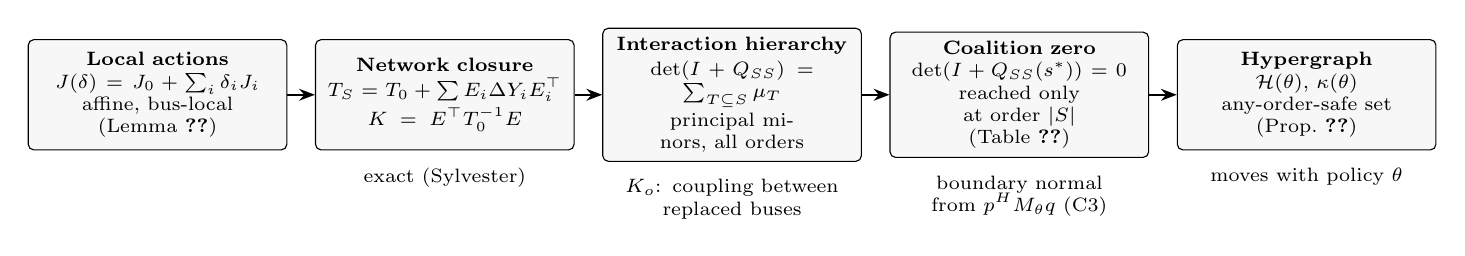
\begin{tikzpicture}[
  node distance=3.5mm,
  box/.style={draw, rounded corners=2pt, align=center, font=\scriptsize,
              minimum height=14mm, text width=30.5mm, fill=gray!6},
  arr/.style={-{Stealth[length=2mm]}, thick}]
\node[box] (a) {\textbf{Local actions}\\ $J(\delta)=J_0+\sum_i\delta_iJ_i$\\ affine, bus-local\\ (Lemma~\ref{lem:affine})};
\node[box, right=of a] (b) {\textbf{Network closure}\\[1pt] $T_S=T_0+\sum E_i\Delta Y_iE_i^{\top}$\\[1pt] $K=E^{\top}T_0^{-1}E$};
\node[box, right=of b] (c) {\textbf{Interaction hierarchy}\\[1pt] $\det(I+Q_{SS})=\sum_{T\subseteq S}\mu_T$\\[1pt] principal minors, all orders};
\node[box, right=of c] (d) {\textbf{Coalition zero}\\ $\det(I+Q_{SS}(s^*))=0$\\ reached only at order $|S|$\\ (Table~\ref{tab:anatomy})};
\node[box, right=of d] (e) {\textbf{Hypergraph}\\ $\Hy(\theta)$, $\kappa(\theta)$\\ any-order-safe set\\ (Prop.~\ref{prop:hierarchy})};
\draw[arr] (a) -- (b); \draw[arr] (b) -- (c); \draw[arr] (c) -- (d); \draw[arr] (d) -- (e);
\node[font=\scriptsize, below=1mm of b, text width=28mm, align=center] {exact (Sylvester)};
\node[font=\scriptsize, below=1mm of c, text width=28mm, align=center] {$K_o$: coupling between replaced buses};
\node[font=\scriptsize, below=1mm of d, text width=28mm, align=center] {boundary normal from $p^HM_\theta q$ (C3)};
\node[font=\scriptsize, below=1mm of e, text width=28mm, align=center] {moves with policy $\theta$};
\end{tikzpicture}
\caption{The chain from local replacement actions to the minimal incompatibility
hypergraph. Each arrow is an exact statement of Section~\ref{sec:closure}; the
IEEE-39 evidence for each box is in Section~\ref{sec:ieee39}.}
\label{fig:chain}
\end{figure*}

% =========================================================================
\section{Model and Problem Formulation}\label{sec:model}

\subsection{Phasor DAE}
The system is the index-one DAE
\begin{equation}\label{eq:dae}
\dot x = f(x,z;\delta,\theta),\qquad 0 = g(x,z;\delta,\theta),
\end{equation}
where $x\in\RR^{n}$ collects device states and $z\in\RR^{2N}$ the rectangular
bus voltages. $g$ is Kirchhoff's current law with the bus admittance matrix,
device injections, and constant-power loads. Index one means that $g_z$ is
nonsingular. At an equilibrium the reduced Jacobian is
$A=f_x-f_z g_z^{-1} g_x$.

\emph{Synchronous generators.} Each SG uses a two-axis model on its own base
\cite{sauer1998}. With $(v_d,v_q)$ the terminal voltage in the rotor frame and
$(i_d,i_q)$ from the stator equations,
\begin{align}
\dot\delta&=\omega_B(\omega-1),\qquad
M\dot\omega=P_m-P_e-D(\omega-1),\label{eq:swing}\\
T'_{d0}\dot e'_q&=e_{fd}-e'_q-(x_d-x'_d)i_d,\nonumber\\
T'_{q0}\dot e'_d&=-e'_d+(x_q-x'_q)i_q,\nonumber
\end{align}
with $P_e=v_di_d+v_qi_q+r_a(i_d^2+i_q^2)$. The AVR is first order,
$T_E\dot e_{fd}=K_A(v_{\rm ref}+v_s-|V|)-e_{fd}$. The stabilizer is a
power-input washout and lag: $v_s=K_Sx_6$, $T_4\dot x_6=T_5(P_e-x_5)/T_6-x_6$,
$T_6\dot x_5=P_e-x_5$. As in the source data, $D=0$ and $P_m$ is constant (no
governor).

\emph{Grid-following inverters.} Each GFL has a synchronous-reference-frame
PLL, filtered power measurements, PI outer loops, and PI inner current loops
behind a filter reactance $x_f$:
\begin{align}
\dot\vartheta&=k_{p,\rm pll}v_q+x_{\rm pll},\qquad \dot x_{\rm pll}=k_{i,\rm pll}v_q,
\label{eq:pll}\\
\tau\dot p_f&=P-p_f,\qquad \tau\dot q_f=Q-q_f,\nonumber\\
i_d^{\rm ref}&=k_p(p_{\rm ref}-p_f)+x_p,\quad
i_q^{\rm ref}=-k_q(q_{\rm cmd}-q_f)-x_q,\nonumber\\
\dot i_{dq}&=\tfrac{\omega_B}{x_f}\big(k_i(i_{dq}^{\rm ref}-i_{dq})+x_{i,dq}-r_fi_{dq}\big),
\nonumber
\end{align}
with PI states $\dot x_p=k_{ip}(p_{\rm ref}-p_f)$,
$\dot x_q=k_{iq}(q_{\rm cmd}-q_f)$, and $\dot x_{i,dq}=k_{ii}(i^{\rm ref}_{dq}-i_{dq})$.
The injection is $\gamma(i_d+ji_q)e^{j\vartheta}$. The reactive command comes
from a leaky Q/V regulator
\begin{align}
q_{\rm cmd}&=k_{p,v}\,g\,e+x_v,\qquad e=v_{\rm ref}-|V|,\label{eq:qv}\\
\dot x_v&= k_{i,v}\,g\,e-w\,(x_v-q_{\rm ref}),\nonumber
\end{align}
with leak $w=0.05$~rad/s; $g=0$ is exact fixed-$Q$ operation. Parameters are
listed in Table~\ref{tab:param}. Converter limits, DC links, and modulation
delay are not modeled.

\begin{table}[!t]
\centering
\caption{Device and benchmark data}\label{tab:param}
\setlength{\tabcolsep}{3pt}
\footnotesize
\begin{tabular}{@{}lL{0.72\columnwidth}@{}}
\toprule
Item & Value (per unit on the device rating) \\
\midrule
SG model & two-axis, power-form swing, $D=0$, constant $P_m$ \\
AVR & $K_A=10.1$, $T_E=0.25$~s (harmonized IEEEX1) \\
PSS & power input: $K_S=-2$, $T_5=1$, $T_6=4.2$, $T_4=0.75$~s \\
PLL & $k_{p,\rm pll}=53$, $k_{i,\rm pll}=1400$ \\
Outer loops & $\tau=0.03$~s; $k_p/k_{ip}=k_q/k_{iq}=0.2/8$ \\
Inner loops & $k_i/k_{ii}=0.25/6$; $x_f=0.15$, $r_f=0.01$ \\
Q/V regulator & $k_{p,v}/k_{i,v}=2/20$; leak $w=0.05$~rad/s; $g\in[0,1]$ \\
Loads & constant power \\
Network & IEEE 39-bus, 46 branches, 10 SGs (bus 39: interconnection) \\
Core & SGs 30, 33, 35, 37 (2096.6~MW; 4270.7~MVA) \\
Census & SGs 30--38 ($2^9=512$ portfolios) \\
\bottomrule
\end{tabular}
\end{table}

\subsection{Replacement portfolios and policy}
Let $V=\{1,\dots,m\}$ be the candidate SGs. A portfolio $S\subseteq V$ has
indicator $\delta_S\in\{0,1\}^m$. Replacing unit $i$ installs a GFL with the
same active and reactive dispatch (\emph{matched dispatch}) and rating equal to
the SG rating, so the AC power flow is identical for every portfolio. The
policy $\theta=(g,k,t,h)$ collects:
\begin{itemize}
\item the Q/V gain $g$;
\item a common scale $k$ of every surviving SG's AVR gain;
\item a scale $t$ of every AVR time constant;
\item a heterogeneity exponent $h$, with $T_{E,i}\mapsto G(T_{E,i}/G)^h$ and
$G$ the geometric mean.
\end{itemize}
Active dispatch (MW) and converter rating (MVA) are reported separately.

% =========================================================================
\section{C1: Transverse Stability and the Minimal Incompatibility Hypergraph}\label{sec:c1}

\begin{assumption}\label{ass:sym}
(i) Every device angle state (rotor angle, PLL angle) enters \eqref{eq:dae}
only through $V e^{-j\,\cdot}$, the other device states are written in their
own rotating frames, and loads and network are rotation-covariant.
(ii) Every SG has $D=0$ and constant $P_m$, and the network is
frequency-independent.
\end{assumption}

Let $R_x$ equal $1$ on every rotor and PLL angle and $0$ elsewhere, and let $w$
be the uniform frequency shift (speed $+1$, PLL integrator $+\omega_B$).

\begin{theorem}[Exact transverse quotient]\label{thm:transverse}
Under Assumption~\ref{ass:sym}(i), $A R_x=0$. Under Assumption~\ref{ass:sym}(i)--(ii),
$A w=\omega_B R_x$, so $C=\spanop\{R_x,w\}$ is $A$-invariant with
$A[R_x\ w]=[R_x\ w]J$, $J=\left[\begin{smallmatrix}0&\omega_B\\0&0
\end{smallmatrix}\right]$ (a Jordan chain). For any orthonormal $Z$ with
$\mathrm{range}\,Z=C^\perp$ and $\Aperp=Z^\top A Z$,
\begin{equation}\label{eq:detid}
\det(sI-A)=s^2\det(sI-\Aperp),
\end{equation}
and $\sigma(\Aperp)$ does not depend on $Z$. The reduced field
$r(x)=f(x,\psi(x))$ satisfies $r(x+\phi R_x)=r(x)$ and
$r(x+c\,w)=r(x)+c\,\omega_B R_x$ for all $\phi,c$, so $\dot y = Z^\top r(x^*+Zy)$
is an exact reduced system with linearization $\Aperp$. With $D\neq0$ or a
governor, only $C=\spanop\{R_x\}$ remains.
\end{theorem}
\begin{proof}
Rotation covariance gives $f(x+\phi R_x,e^{j\phi}z)=f(x,z)$ and a covariant
$g$. Differentiating at $\phi=0$ gives $f_xR_x+f_zR_z=0$ and $g_xR_x+g_zR_z=0$
with $R_z=jV$, so $AR_x=0$. Under (ii), $x_0+c\,w+c\,\omega_B tR_x$ with
$z(t)=e^{jc\omega_B t}z_0$ solves \eqref{eq:dae} exactly, and differentiating
in $c$ gives $Aw=\omega_BR_x$. In the basis $[U\ Z]$, with $U$ an orthonormal
basis of $C$, invariance gives $Z^\top AU=0$. $A$ is then block triangular with
diagonal blocks $U^\top AU$ (spectrum $\{0,0\}$) and $\Aperp$, which yields
\eqref{eq:detid}. A different complement $ZO$ gives $O^\top\Aperp O$. The
nonlinear identities are proved in Appendix~\ref{app:proofs}.
\end{proof}

\begin{definition}\label{def:stable}
$S$ is \emph{transversely stable} at $\theta$ if
$\aperp(S,\theta)=\max\mathrm{Re}\,\sigma(\Aperp(S,\theta))<0$.
\end{definition}

The rotation is a gauge. The drift is a physical consequence of absent primary
frequency control, so transverse stability is stability modulo absolute
frequency restoration. The magnitude cutoff ``ignore $|\lambda|\le\varepsilon$''
agrees with Definition~\ref{def:stable} only when $\Aperp$ has no physical
eigenvalue in that disc. In suite S1 (Section~\ref{sec:mc}) it miscounts all
235 draws with a planted positive physical mode of size
$10^{-5}$--$5\times10^{-4}$, and none of the others.

\emph{Numerical labels.} Every label is produced without a magnitude cutoff.
\begin{enumerate}
\item The AC equilibrium is solved to a residual below $10^{-12}$, and the
Jacobians are formed by central differences at steps $h$ and $2h$, whose
difference gives the error $E$.
\item $R_x$ and $w$ are verified ($\|AR_x\|$, $\|Aw-\omega_BR_x\|$), and
$\Aperp$ and $E_\perp=Z^\top EZ$ are formed.
\item If $\min|\mathrm{Re}\,\sigma(\Aperp)|>2\times10^{-3}$~s$^{-1}$, the label
is the sign of $\aperp$.
\item Otherwise the label is exact if
$d=\min_\omega\sigma_{\min}(\Aperp-j\omega I)>10\varepsilon$, with
$\varepsilon=\|E_\perp\|+$ backward error. If not, the point is
\textsc{unresolved}: reported, never assigned.
\end{enumerate}
This is a numerical criterion, not an interval certificate.

\begin{definition}\label{def:hyper}
For fixed $\theta$ with a transversely stable base, let
$\mathcal{U}(\theta)=\{S:\aperp(S,\theta)\ge 0\}$. The \emph{minimal
incompatibility hypergraph} $\Hy(\theta)$ is the family of inclusion-minimal
elements of $\mathcal{U}(\theta)$, and $\kappa(\theta)=\min_{e\in\Hy}|e|$, with
$\kappa=\infty$ if $\Hy=\emptyset$.
\end{definition}

\begin{proposition}[Structure]\label{prop:structure}
$\Hy(\theta)$ is an antichain, and a portfolio containing no hyperedge is
transversely stable. $\mathcal{U}$ need not be upward closed.
\end{proposition}
\begin{proof}
Minimal elements form an antichain. If $S$ is unstable, a minimal unstable
subset of $S$ is a hyperedge contained in $S$.
\end{proof}

For a target $T$, define three planning predicates:
\begin{itemize}
\item \textbf{A}: $T$ is stable.
\item \textbf{B}: some one-at-a-time chain
$\emptyset=S_0\subset\dots\subset S_{|T|}=T$ has every $S_j$ stable.
\item \textbf{C}: every $R\subseteq T$ is stable, so every implementation order
passes only through stable stationary states.
\end{itemize}

\begin{proposition}[Any-order safety]\label{prop:hierarchy}
C $\Rightarrow$ B $\Rightarrow$ A, and neither converse holds in general. With a
stable base, $T$ satisfies C iff $T$ contains no hyperedge of $\Hy(\theta)$.
\end{proposition}
\begin{proof}
C gives any chain, and B ends at $T$. $T$ violates C iff some $R\subseteq T$ is
unstable, iff (Proposition~\ref{prop:structure}) a hyperedge lies in $T$.
\end{proof}
For A without B, take diagonal vertices $A_\emptyset=-I$,
$A_{\{1\}}=\mathrm{diag}(2,-3)$, $A_{\{2\}}=\mathrm{diag}(-3,2)$, and
$A_{\{1,2\}}=-2I$. For B without C, one proper subset is unstable while
another chain avoids it.

\begin{theorem}[Boundary localization]\label{thm:localization}
Let $\theta(\tau)$ be continuous with $g_z$ nonsingular along the path for every
portfolio, and let Assumption~\ref{ass:sym} hold. Then $\Hy(\theta(\tau))$ is
constant on every interval on which no $\Aperp(S,\theta(\tau))$ has an
eigenvalue on the imaginary axis. Every change of $\Hy$ is bracketed by such a
crossing, at finite frequency or at $s=0$.
\end{theorem}
\begin{proof}
$\Aperp(S,\theta(\tau))$ is continuous because $g_z^{-1}$ is, so its
eigenvalues are continuous. The sign of $\aperp$ can change only through
$\mathrm{Re}\,\lambda=0$, and $\Hy$ is a function of the $2^m$ labels.
\end{proof}

\emph{Supporting results.} Two further statements are credited to known
theory.
\begin{itemize}
\item \emph{Monotone class.} If a common similarity makes every
$T^{-1}A(S)T$ Metzler and order-preserving in $S$, then $\aperp$ is monotone
on the lattice and A $=$ B $=$ C \cite{farina2000positive}. One robust pair
$S\subset S'$ with $\aperp(S)>0>\aperp(S')$ excludes every such realization.
\item \emph{Complexity.} Deciding whether some $|S|\le k$ destabilizes is
NP-complete, already for $D_\delta WD_\delta-(k-1)I$ with $W$ a graph adjacency
matrix. This is the clique reduction behind sparse PCA
\cite{karp1972, magdon2017sparsepca}; see also
\cite{poljak1993robust, nemirovskii1993robust, katewa2020sparse}.
\end{itemize}
\label{prop:monotone}\label{prop:complexity}

% =========================================================================
\section{C2 and C3: Network Closure and Boundary Motion}\label{sec:closure}

\subsection{Local actions: a descriptor realization affine in the indicators}
Under matched dispatch, every candidate bus can carry \emph{both} devices: the
SG with weight $(1-\delta_i)$ and the GFL with weight $\delta_i$. An absent
device is replaced by a stable filler $\dot x=-(x-x_0)$ at its intensive
equilibrium, which is common to all vertices.

\begin{lemma}\label{lem:affine}
On this realization the descriptor Jacobian is exactly affine,
$J(\delta)=J_0+\sum_i\delta_iJ_i$. Each $J_i$ is supported on the states of the
devices at bus $i$ and on the two voltage channels of bus $i$.
\end{lemma}
The weights multiply injections only. Each vertex has the spectrum of the
actual portfolio plus the fillers' $-1$ eigenvalues. The reduced $A(\delta)$
is \emph{not} affine, because $g_z$ depends on $\delta$.

\subsection{Network closure and the interaction hierarchy}
Keep the network variables and eliminate only the device states:
$T_S(s)=g_z+g_x(sI-f_x)^{-1}f_z$ at $\delta_S$. Let $E$ select the $2m$
voltage channels of the candidate buses, and define
$\Delta Y_i(s)=E_i^\top(T_{\{i\}}-T_0)E_i$ ($2\times 2$),
$D=\blkdiag(\Delta Y_i)$, and $K=E^\top T_0^{-1}E$. Split $K=K_d+K_o$ into its
$2\times2$ diagonal blocks and the off-diagonal blocks, which carry the network
coupling between the replaced buses. Set
\begin{equation}\label{eq:Q}
M=DK,\qquad Q=(I+DK_d)^{-1}DK_o .
\end{equation}

\begin{theorem}[Network-closure factorization]\label{thm:factorization}
Let $s$ be neither a device pole nor a zero of $\det T_0$. For every $S$,
\begin{align}
\det P_S(s)&=h_S(s)\,\det T_0(s)\,\det\!\big(I+M_{SS}(s)\big),\label{eq:fact1}\\
\det\!\big(I+M_{SS}\big)&=\prod_{i\in S}\det(I+M_{ii})\;\det\!\big(I+Q_{SS}\big),
\label{eq:fact2}
\end{align}
where $P_S$ is the descriptor pencil and $h_S=\det(sI-f_x)$ is a product of
per-device factors. Moreover $\det(I+Q_{SS})=\sum_{T\subseteq S}\mu_T$ with
$\mu_\emptyset=1$, $\mu_{\{i\}}=0$, and, for $|T|\ge2$,
\begin{equation}\label{eq:mu}
\mu_T=\sum_{U:\ \mathrm{blocks}(U)=T}\det Q_{UU},
\end{equation}
the sum of the principal minors of $Q$ that touch exactly the blocks of $T$.
$\mu_T$ is the M\"obius coefficient of $S\mapsto\det(I+Q_{SS})$ and is
invariant under block-diagonal changes of port basis.
\end{theorem}
\begin{proof}
The Schur complement gives $\det P_S=h_S\det T_S$. By Lemma~\ref{lem:affine},
$T_S=T_0+\sum_{i\in S}E_i\Delta Y_iE_i^\top$ exactly (Appendix~\ref{app:proofs}),
and Sylvester's identity gives \eqref{eq:fact1}. Since $I+DK_d$ is block
diagonal, $I+M_{SS}=(I+DK_d)_{SS}(I+Q_{SS})$, which gives \eqref{eq:fact2}.
Multilinearity gives $\det(I+X)=\sum_U\det X_{UU}$, and grouping minors by the
blocks they touch gives \eqref{eq:mu}. Since $Q_{ii}=0$, $\mu_{\{i\}}=0$.
M\"obius inversion is unique \cite{rota1964mobius}, and a block-diagonal
similarity leaves every $\det(I+Q_{SS})$ unchanged.
\end{proof}

\begin{corollary}[Boundaries are network-closure zeros]\label{cor:closure}
If no member of $S$ alone and no device has an eigenvalue at $s^*$, then
$s^*\in\sigma(\Aperp(S))$ iff $-1\in\sigma(M_{SS}(s^*))$ iff
$\det(I+Q_{SS}(s^*))=0$. With $K_o=0$ no such $s^*$ exists.
\end{corollary}

Every non-additive effect of a replacement portfolio is therefore an
interaction term $\mu_T$ generated by network closure between the replaced
buses. The algebraic degree of $S\mapsto\det(I+Q_{SS})$ and $\kappa$ are
different quantities: an affine family can have $\kappa=m$, and a full-degree
family can have $\kappa=1$. The theorem does not say which order closes a given
boundary; that is measured in Section~\ref{sec:ieee39}.

\emph{Why aggregate indices fail.} Aggregate displaced dispatch, and any other
function of per-unit data, is blind to the off-diagonal blocks $K_o$. It
therefore removes the dynamic interaction geometry contained in $Q_{SS}$ and
its principal minors, which by \eqref{eq:fact2} carry the entire non-additive
part of the characteristic function.

\subsection{Boundary motion (C3)}
\begin{proposition}[Boundary sensitivity]\label{prop:gradient}
Let $-1$ be a simple eigenvalue of $M_{SS}(s^*,\theta^*)$ with right and left
eigenvectors $q,p$. Then
\begin{equation}\label{eq:grad}
\frac{\partial s^*}{\partial\theta}=
-\frac{p^{H}\,\partial_\theta M_{SS}\,q}{p^{H}\,\partial_s M_{SS}\,q},
\end{equation}
and $\nabla_\theta\,\mathrm{Re}\,s^*$ is the normal of the boundary.
\end{proposition}
\begin{proof}
Simple-eigenvalue perturbation gives $d\lambda=p^{H}dM\,q/p^{H}q$. The implicit
function theorem applied to $\lambda(s,\theta)=-1$ yields \eqref{eq:grad}.
\end{proof}

\emph{Zero-frequency crossings.} By \eqref{eq:detid}, $\det T_S(0)$ vanishes
structurally for every $S$, so the port test is blind to aperiodic crossings.
Let $U=R_x/\|R_x\|$ and $\beta,\beta_2>0$, and relocate
$f_x^{\#}=f_x-\beta UU^\top$. The vector $x_0=w+aR_x$ with
$a=\omega_B/\beta-U^\top w/\|R_x\|$ is then a null vector of the relocated
reduced matrix. Set $f_x^{\#\#}=f_x^{\#}-\beta_2x_0x_0^\top/\|x_0\|^2$ and
$T^{\#\#}(0)=g_z-g_x(f_x^{\#\#})^{-1}f_z$.

\begin{theorem}[Symmetry-deflated zero-frequency port]\label{thm:port}
$\sigma(A^{\#\#})=\sigma(\Aperp)\cup\{-\beta,-\beta_2\}$ and
$\det T^{\#\#}(0)=\det g_z\det A^{\#\#}/\det f_x^{\#\#}$. Along a path on which
$\mathrm{sign}\det g_z$ and $\mathrm{sign}\det f_x^{\#\#}$ are constant,
$\mathrm{sign}\det T^{\#\#}(0)$ changes iff the number of positive real
eigenvalues of $\Aperp$ changes parity.
\end{theorem}
\begin{proof}
Brauer's rank-one theorem \cite{brauer1952} moves one zero to $-\beta$. The
Jordan partner becomes the exact null vector $x_0$, which a second rank-one
update moves to $-\beta_2$. The identity is the Schur formula. Complex pairs
contribute $|\lambda|^2>0$, so
$\mathrm{sign}\det\Aperp=(-1)^{\dim\Aperp}(-1)^{\#\{\lambda>0\}}$.
\end{proof}
The test does not see complex crossings, which are covered by \eqref{eq:fact1}.
It also does not see coalescences of two positive real eigenvalues, in which
nothing crosses $s=0$.

% =========================================================================
\section{IEEE 39-Bus Evidence}\label{sec:ieee39}

\subsection{Benchmark}
The IEEE 39-bus system \cite{athay1979} is taken from the ANDES dynamic case
\cite{cui2021andes, andes_ieee39_dynamic_case}, with ten two-axis SGs; bus~39
represents the interconnection and is never replaced. The documented IEEEX1
exciter is harmonized into a first-order AVR (regulator gain, exciter time
constant), which is a declared model change. The core candidates are SGs 30,
33, 35, and 37; replacing all four displaces 2096.6~MW of active dispatch on
4270.7~MVA of converter rating. Every result is conditional on this model.

\subsection{C1: policy-dependent minimal incompatibility}
Three policy planes were mapped: F7A ($g\times k$), F7B ($g\times t$), and F7C
($g\times h$). All 345\,229 points were re-audited in transverse coordinates on
the direct path. No resolved label changed, and 1.5\% of the points remain
within the classifier's numerical resolution. The planes carry 30, 36, and 16
distinct hypergraphs, with up to 15 hypergraphs behind a single value of
$\kappa$ (Fig.~\ref{fig:map}).
\begin{itemize}
\item At the reference point P4 ($g=0.03625$, $k=1.425$, $t=1.5$, $h=1$),
$\Hy=\{\{30,33,35,37\}\}$ and $\aperp=+0.127$~s$^{-1}$: every proper subset is
stable and the four-unit portfolio is not.
\item At full voltage-support gain (P$_\infty$: $g=1$, $k=0.5$),
$\Hy=\emptyset$.
\item On the line $t=0.852$, the minimal witness contracts $4\to3\to2$ and
re-expands $3\to4\to\emptyset$ as $g$ increases (Fig.~\ref{fig:path}).
\end{itemize}

\begin{figure}[!t]
\centering
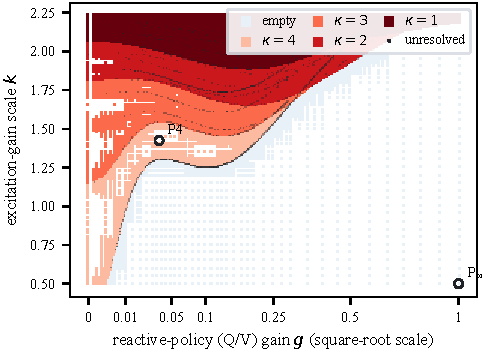
\includegraphics[width=\columnwidth]{fig_policy_map.pdf}
\caption{Transverse minimum incompatible order $\kappa$ over the F7A policy plane
of IEEE-39 ($t=1.5$, $h=1$, core 30/33/35/37, matched dispatch, no governor).
Black dots: points within classifier resolution.}
\label{fig:map}
\end{figure}

\emph{Primary frequency control.} The same source workbook documents TGOV1N
turbine governors ($R=0.05$, $T_1=0.05$, $T_2=1$, $T_3=2.1$~s). They were added
untuned as a separately versioned model, for which $C=\spanop\{R_x\}$
(Theorem~\ref{thm:transverse}). Fig.~\ref{fig:gov} and Table~\ref{tab:gov} show
the result:
\begin{itemize}
\item The P4 four-unit portfolio becomes stable ($\aperp=-0.0745$), although it
remains the least-damped portfolio of the lattice.
\item On a 399-point plane the number of distinct hypergraphs falls from 26 to
10. Non-empty structure remains at 74 points ($\kappa=2,3,4$), no singleton
fails, and the base is always stable.
\item The re-entrant tongue on $k=1.30$ disappears.
\item In ANDES the governors move the base inter-area pair from $-0.222$ to
$-0.770$~s$^{-1}$, which is consistent in direction.
\end{itemize}
The specific four-unit witness is conditional on the absence of primary
frequency control, while policy-dependent incompatibility persists in the
governed model in a smaller region. $\Hy$ is a property of the system and
policy, not a permanent label on buses.

\begin{figure}[!t]
\centering
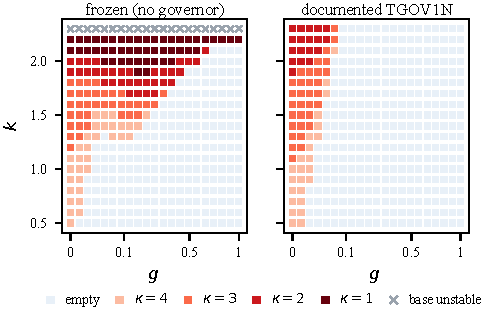
\includegraphics[width=\columnwidth]{fig_governed.pdf}
\caption{Minimum incompatible order on a coarse IEEE-39 policy plane ($t=1.5$,
$h=1$): frozen model versus the model with the source's documented TGOV1N
governors.}
\label{fig:gov}
\end{figure}

\begin{table}[!t]
\centering
\caption{Frozen versus governed IEEE-39 (documented TGOV1N)}\label{tab:gov}
\setlength{\tabcolsep}{3pt}
\footnotesize
\begin{tabular}{@{}L{0.34\columnwidth}L{0.29\columnwidth}L{0.29\columnwidth}@{}}
\toprule
Quantity & Frozen & Governed \\
\midrule
P4 four-unit $\aperp$ & $+0.127$ & $-0.0745$ \\
P4 line, $\kappa=4$ window & $g\in[0.016,0.20]$ & $g\in[0.016,0.023]$ \\
tongue line $k=1.30$ & U--S--U--S (re-entry) & no re-entry \\
plane: distinct $\Hy$ & 26 & 10 \\
plane: non-empty points & 148 (+21 base unstable) & 74 (base always stable) \\
plane: $\kappa=1$ points & 48 & 0 \\
reference points non-empty & 5 of 6 & 1 of 6 (P3) \\
damped condenser, P4 & threshold 2.48--3\% & not needed \\
\bottomrule
\end{tabular}
\end{table}

\emph{Displaced MW is not the variable.} The failing mode is the
0.64--0.71~Hz inter-area family (Fig.~\ref{fig:dispatch}). The 25 stable
four-unit census portfolios whose displaced dispatch matches that of the 10
unstable ones all keep the family damped
($\max\mathrm{Re}\le-0.114$~s$^{-1}$, $\zeta\ge3.9\%$). The family is unstable in
8 of the 10 failing portfolios, and total displaced dispatch predicts the
minimal coalition with AUC 0.57. Section~\ref{sec:closure} explains why: MW is
blind to the interaction geometry in $Q_{SS}$.

\begin{figure}[!t]
\centering
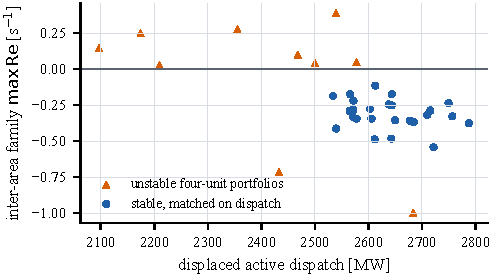
\includegraphics[width=\columnwidth]{fig_dispatch.pdf}
\caption{Inter-area family abscissa versus displaced active dispatch for the
unstable four-unit census portfolios and 25 stable portfolios matched on
dispatch.}
\label{fig:dispatch}
\end{figure}

\subsection{C2: network-closure anatomy of ten frozen boundaries}
Ten frozen boundaries were re-located by bisection and analyzed with
Theorem~\ref{thm:factorization}: the nine witness changes of the F7B line
$t=0.852$, and the four-unit boundary on the P4 line ($g^*=0.2077$, 0.706~Hz).
\begin{itemize}
\item \emph{Local actions.} The descriptor blocks $f_x,f_z,g_x,g_z$ are affine
in $\delta$ to $4.5\times10^{-16}$ (order-$\ge2$ M\"obius coefficients). Each
replacement touches only its own devices and bus.
\item \emph{Exact closure.} \eqref{eq:fact1} holds to $1.4\times10^{-13}$ for
all 16 subsets at all ten points, and the critical eigenvalue of $M_{SS}$
equals $-1$ to $8.5\times10^{-14}$.
\item \emph{Local factor never vanishes.} $\prod_i\det(I+M_{ii})$ stays between
0.08 and 0.31. The zero is carried entirely by $\det(I+Q_{SS})$.
\end{itemize}

The central result is the following observation (Table~\ref{tab:anatomy},
Fig.~\ref{fig:closure}). \emph{For every one of the ten frozen IEEE-39
boundaries, no interaction truncation below the cardinality of the changing
minimal coalition reaches the characteristic zero.} Truncating at order $|S|-1$
leaves 0.29--0.40 for the triples and 0.13--0.16 for the four-unit portfolio,
whereas the full order reaches $\le4\times10^{-13}$. Table~\ref{tab:orders}
shows the build-up at the four-unit boundary. The interaction coefficients of
orders 2, 3, and 4 have comparable magnitude (0.51, 0.45, and 0.16). The
fourth-order term, a sum of principal minors of $Q$ that touch all four
replaced buses, is exactly what closes the determinant. Across 120 random
$(\theta,s)$ draws (suite P3), the full-order coefficient never vanishes
($7.8\times10^{-4}$ to 469), so no lower-degree representation is exact on this
benchmark.

\begin{table}[!t]
\centering
\caption{Network-closure anatomy of ten frozen IEEE-39 boundaries}\label{tab:anatomy}
\setlength{\tabcolsep}{2.4pt}
\footnotesize
\begin{tabular}{@{}llrrrrrrr@{}}
\toprule
Ev. & $S$ changing & $g^*$ & Hz & local & trunc.$^{a}$ & $\sigma_1(Q)$ & rank$^{b}$ & angle$^{c}$\\
\midrule
E1 & 30+33+35 & 0.0102 & 0.628 & 0.315 & 0.336 & 6.13 & 7 & 2.3e-4\\
E2 & 30+33+37 & 0.0188 & 0.633 & 0.198 & 0.396 & 6.88 & 7 & 7.1e-5\\
E3 & 33+35+37 & 0.0609 & 0.671 & 0.080 & 0.385 & 4.00 & 8 & 2.7e-4\\
E4 & 30+33 & 0.1034 & 0.656 & 0.081 & 1 & 8.93 & 7 & 1.8e-4\\
E5 & 33+35+37 & 0.1870 & 0.695 & 0.135 & 0.296 & 2.37 & 8 & 3.3e-4\\
E6 & 30+33 & 0.2491 & 0.672 & 0.104 & 1 & 6.06 & 7 & 8.4e-5\\
E7 & 30+33+35 & 0.2778 & 0.706 & 0.130 & 0.372 & 2.01 & 8 & 3.5e-4\\
E8 & 30+33+37 & 0.2931 & 0.685 & 0.132 & 0.293 & 3.46 & 8 & 2.0e-4\\
E9 & 30+33+35+37 & 0.2973 & 0.718 & 0.134 & 0.132 & 1.67 & 8 & 2.9e-4\\
F & 30+33+35+37 & 0.2077 & 0.706 & 0.089 & 0.161 & 1.84 & 8 & 4.3e-4\\
\bottomrule
\end{tabular}\\[2pt]
\footnotesize E1--E9: F7B line $t=0.852$ ($k=h=1$); F: P4 line ($k=1.425$,
$t=1.5$). $^{a}|\det(I+Q_{SS})|$ truncated at order $|S|-1$ (for pairs this is
order 1, which is identically 1); the full order gives $\le4\times10^{-13}$.
$^{b}$Effective rank of $Q$ at $10^{-2}$. $^{c}$Boundary-normal error of
\eqref{eq:grad} against direct finite differences [deg].
\end{table}

\begin{figure}[!t]
\centering
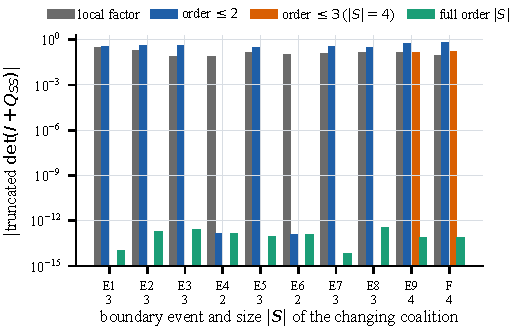
\includegraphics[width=\columnwidth]{fig_closure.pdf}
\caption{Anatomy of the ten frozen IEEE-39 boundaries (E1--E9: F7B line
$t=0.852$; F: P4 line). Shown are the local factor and the truncations of the
interaction expansion \eqref{eq:mu}. Only the full-order term (order $|S|$)
reaches the characteristic zero. For pairs, order $\le2$ is the full order.}
\label{fig:closure}
\end{figure}

\begin{table}[!t]
\centering
\caption{Order-by-order expansion at the four-unit boundary (P4 line, 0.706~Hz)}\label{tab:orders}
\setlength{\tabcolsep}{4pt}
\footnotesize
\begin{tabular}{@{}crrrr@{}}
\toprule
& \multicolumn{2}{c}{$\det(I+M_{SS})$} & \multicolumn{2}{c}{$\det(I+Q_{SS})$}\\
\cmidrule(lr){2-3}\cmidrule(lr){4-5}
Order $k$ & $|\sum_{|T|=k}\mu_T|$ & $|$trunc.\ $\le k|$ & $|\sum_{|T|=k}\tilde\mu_T|$ & $|$trunc.\ $\le k|$\\
\midrule
0 & 1 & 1 & 1 & 1\\
1 & 2.509 & 1.712 & 0 & 1\\
2 & 2.393 & 0.889 & 0.509 & 0.605\\
3 & 0.989 & 0.146 & 0.445 & 0.161\\
4 & 0.146 & $7\times10^{-15}$ & 0.161 & $8\times10^{-14}$\\
\bottomrule
\end{tabular}\\[2pt]
\footnotesize The left pair includes the local terms; in the right pair they
are factored out ($\tilde\mu_{\{i\}}=0$, Theorem~\ref{thm:factorization}).
\end{table}

\emph{Negative control: interaction dimension.} The effective rank of $Q$
(threshold $10^{-2}$) stays at 7--8 of 8 while $\kappa$ changes
$4\to3\to2\to3\to4$ (Fig.~\ref{fig:path}). Interaction dimension is therefore
not the mechanism of witness contraction, and we do not claim that rank
explains $\kappa$. The magnitude $\sigma_1(Q)$ varies (6.1--8.9 at the
contracting events, 1.7--1.8 at the four-unit boundaries), but this is only
descriptive.

\begin{figure}[!t]
\centering
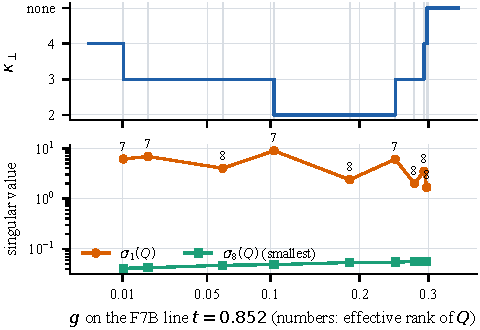
\includegraphics[width=\columnwidth]{fig_path.pdf}
\caption{F7B policy line $t=0.852$. Top: the transverse minimum incompatible
order contracts $4\to3\to2$ and re-expands. Bottom: largest and smallest singular
values of $Q$ at the nine boundary events, labelled with the effective rank. The
dimension stays full while $\kappa$ changes (negative control).}
\label{fig:path}
\end{figure}

\emph{Limitation: no path attribution.} A bus-diagonal Neumann walk expansion of
$T_0^{-1}$ ($T_0=D_g-N$) does not converge in the inter-area band
($\rho(D_g^{-1}N)\ge1.003$ over 0.3--1.5~Hz), both at the four-unit boundary
and for a Pg-matched stable control. No n-hop attribution is claimed. The
closure result concerns the order of the interaction, not a dominant path or
cycle; the simple-cycle explanation was tested separately and falsified.

\subsection{C3: boundary motion, retuning, and zero-frequency crossings}
Formula \eqref{eq:grad} was compared with direct finite differences of the
tracked transverse eigenvalue in all four policy coordinates. At all ten
boundaries the boundary normal agrees to $4.3\times10^{-4}$~degrees, its
magnitude to $4.3\times10^{-6}$ (relative), and the frequency drift to
$9\times10^{-6}$ (Table~\ref{tab:anatomy}).

Consider making the P4 portfolio stable by a pure Q/V-gain change
(Fig.~\ref{fig:retune}). A single linear step predicts $\Delta g=0.052$, whereas
continuation gives $0.171$: the slope $\partial\,\mathrm{Re}\,s/\partial g$
drifts from $-2.45$ at P4 to $-0.46$ at the boundary. Newton iteration with
\eqref{eq:grad} reaches the continuation boundary $g^*=0.20768$ to
$2\times10^{-10}$ in five steps. The port derivative is therefore an exact local
tool and an iterative retuning tool, not a one-shot predictor.

\begin{figure}[!t]
\centering
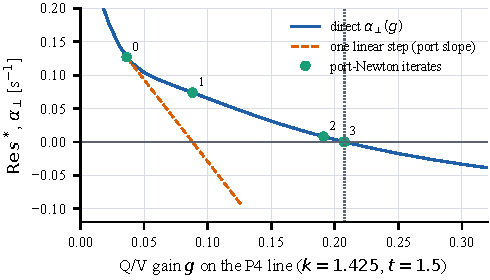
\includegraphics[width=\columnwidth]{fig_retune.pdf}
\caption{Q/V retuning of the P4 four-unit portfolio. The single linear step
built from the port derivative \eqref{eq:grad} undershoots because the slope
changes fivefold along the path. Newton iteration with the same derivative
reaches the continuation boundary (dotted) to $2\times10^{-10}$.}
\label{fig:retune}
\end{figure}

IEEE-39 has no real transverse crossing, so Theorem~\ref{thm:port} is exercised
on the Kundur two-area system. There, all 194 aperiodic crossings of the
policy maps are leaky Q/V-integrator modes passing through $s=0$. These 194
motivated the construction and are not counted as validation. The frozen
construction was then evaluated on held-out Kundur slices (Fig.~\ref{fig:port}):
\begin{itemize}
\item actual zero-frequency crossings: 28, detected 28/28;
\item one further real-count change is a coalescence of two positive real
eigenvalues into a complex pair, correctly not a zero-crossing event;
\item false positives on 445 controls (109 oscillatory crossings, 336
no-crossing brackets): 0.
\end{itemize}

\begin{figure}[!t]
\centering
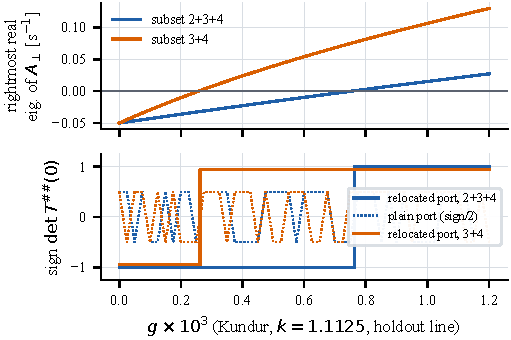
\includegraphics[width=\columnwidth]{fig_port.pdf}
\caption{Symmetry-deflated zero-frequency port on a Kundur holdout line. Top:
the physical real transverse eigenvalue crosses zero. Bottom: the relocated
port changes sign exactly at the crossings; the plain port (dotted) is
structurally singular and its sign is numerical noise.}
\label{fig:port}
\end{figure}

\subsection{Planning consequences}\label{sec:planning}
Proposition~\ref{prop:hierarchy} is exact, so $\Hy$ becomes a set-packing
constraint for any-order-safe portfolios (Table~\ref{tab:planning}).
\begin{itemize}
\item Order dependence exists but is rare. On the 512-portfolio census at one
reference policy, 327 portfolios are stable and 3 of these are
order-dependent; each becomes unsafe exactly when unit 34 is converted last.
On the P2 random paths, 131 of 30\,755 stable targets are order-dependent.
\item The three census pairs also exclude the monotone class.
\item The MW-optimal census plan (3652.3~MW / 6499.9~MVA) is safe in any order.
\end{itemize}
Sequencing is therefore not the dominant application. The main planning use is
the any-order-safe set and its movement with policy.

A damped condenser restores P4 above 2.48\% of the retired rating
(106.0~MVA). Keeping a 200-MW disturbance inside the declared converter voltage
band requires 684--792~MVA; this is an envelope requirement of the model, not
a stability requirement.

\begin{table}[!t]
\centering
\caption{Planning results on IEEE-39 (MW and MVA on separate axes)}\label{tab:planning}
\setlength{\tabcolsep}{3pt}
\footnotesize
\begin{tabular}{@{}L{0.23\columnwidth}L{0.22\columnwidth}L{0.49\columnwidth}@{}}
\toprule
Problem & Setting & Result \\
\midrule
Any-order safe & core, P4 & 30+33+35: 1775.1~MW / 3300.5~MVA\\
Any-order safe & core, P$_\infty$ & 30+33+35+37: 2096.6~MW / 4270.7~MVA\\
Any-order safe & 9-unit census & 31+32+34+35+37+38: 3652.3~MW / 6499.9~MVA\\
Order dependence & 9-unit census & 3 of 327 stable targets\\
Nonlinear safe & core, P4 & out of model scope\\
Nonlinear safe & core, P$_\infty$, D2 & identical to spectral\\
Support & P4, small signal & 106.0~MVA (damped condenser)\\
Support & P4, envelope & 684--792~MVA (not a stability requirement)\\
Governors & P4 & stable without support\\
\bottomrule
\end{tabular}
\end{table}

% =========================================================================
\section{Monte Carlo Validation (Supporting)}\label{sec:mc}

All pass rules were frozen in a configuration file committed before any draw.
Synthetic suites S1--S7 draw random systems that satisfy exactly one
statement's hypotheses (Appendix~\ref{app:mc}). The IEEE-39 suites P1--P4 draw
random policies ($g=u^2$, $u\sim U(0,1)$; $k\in[0.5,2.3]$; $t\in[0.5,3]$;
$h\in[0,2]$) and random portfolios of the core:
\begin{itemize}
\item P1 checks Theorem~\ref{thm:transverse}, including the nonlinear
symmetries at random off-equilibrium states;
\item P2 follows random policy segments and re-brackets every change of $\Hy$;
\item P3 checks \eqref{eq:fact1} and \eqref{eq:mu} at random $s$;
\item P4 compares nonlinear TDS (5-MW pulse) with the sign of $\aperp$ on 40
stable and 40 unstable draws.
\end{itemize}
Table~\ref{tab:mc} and Fig.~\ref{fig:mc} report the results. Checks that are
logical identities validate the implementation; the informative outputs are the
physical checks and the frequencies.

All preregistered IEEE-39 checks passed except the P2 localization tolerance
rule, which failed as implemented; its post-hoc re-bisection is reported
separately. \PtwoText{} The TDS envelope rate tracks $\aperp$ ($r=0.969$),
which confirms that Definition~\ref{def:stable} is the stability notion the
nonlinear model obeys. The synthetic frequencies show that the converses of
Proposition~\ref{prop:hierarchy} fail often in random families (65\% have a
stable target that is not safe in every order, and 4\% have one that is
unreachable by any safe path), and that the monotone class is narrow (99.7\% of
sign-unconstrained families violate it).

\begin{table*}[!t]
\centering
\caption{Preregistered Monte Carlo validation}\label{tab:mc}
\setlength{\tabcolsep}{3.5pt}
\footnotesize
\begin{tabular}{@{}L{2.7cm}L{1.75cm}rL{1.45cm}L{6.35cm}L{3.0cm}@{}}
\toprule
Statement & Suite & Draws & $N$ & Measured & Frozen rule / result \\
\midrule
Thm~\ref{thm:transverse} (linear) & S1 synthetic & 1000 & 1000 & exact RHP count 1000/1000; \eqref{eq:detid} $\le 5.5\!\times\!10^{-9}$; basis $1.5\!\times\!10^{-16}$ & $\le 10^{-8}$: pass\\
\quad control: magnitude cutoff & S1 & 1000 & 1000 & wrong in 235/235 positive planted modes, 0/765 otherwise & expected failure: confirmed\\
Props~\ref{prop:structure},\ref{prop:hierarchy} & S2 synthetic & 2000 & 30\,881 targets & 0 violations; A$\setminus$B in 86 families, B$\setminus$C in 1276 & 0 violations: pass\\
Thm~\ref{thm:localization} & S3 synthetic & 300 & 1044 crossings & every $\Hy$ change bracketed (698 real, 346 complex) & 0 exceptions: pass\\
monotone class & S4 synthetic & 1000 & 80\,000 edges & 0 non-monotone edges, A$=$B$=$C & pass\\
\quad control: signs removed & S4 & 1000 & 80\,000 & 37\,166 non-monotone edges in 997/1000 families & expected failure: confirmed\\
complexity & S5 synthetic & 500 & exhaustive & 0 mismatches with $k$-cliques & pass\\
Thm~\ref{thm:factorization} (algebra) & S6 synthetic & 500 & 500 & minors $3.4\!\times\!10^{-15}$, M\"obius $1.3\!\times\!10^{-15}$, invariance $8.2\!\times\!10^{-12}$ & $\le 10^{-10}$: pass\\
Thm~\ref{thm:port} & S7 synthetic & 1000 & 817 decided & flip $\Leftrightarrow$ parity change in 817/817; 183 undecided by the device-flip rule & pass$^{a}$\\
\midrule
Thm~\ref{thm:transverse} (physical) & P1 IEEE-39 & 300 & 300 & $\dim C=2$ in 300/300; spectrum $4.5\!\times\!10^{-9}$; Jordan entry $3.9\!\times\!10^{-12}$ & pass\\
Thm~\ref{thm:transverse} (nonlinear) & P1 IEEE-39 & 300 & 300 & $r(x\!+\!\phi R_x)$: $2.4\!\times\!10^{-14}$; $r(x\!+\!cw)$: $9.4\!\times\!10^{-15}$ & $\le 10^{-8}$: pass\\
Thm~\ref{thm:localization}, Prop~\ref{prop:hierarchy} & P2 IEEE-39 & \PtwoSegments{} paths & \PtwoCrossings{} & \PtwoResult & \PtwoPass\\
Thm~\ref{thm:factorization} (physical) & P3 IEEE-39 & 40 & 120 & ratio $3.2\!\times\!10^{-13}$; M\"obius $8.1\!\times\!10^{-13}$ & $\le 10^{-8}$: pass\\
Def.~\ref{def:stable} in TDS & P4 IEEE-39 & 80 & 80 & TDS verdict $=$ sign of $\aperp$ in 80/80; rate vs.\ $\aperp$: $r=0.969$ & 80/80: pass\\
Thm~\ref{thm:port} (physical) & Kundur holdout & 474 & 28$+$445 & zero crossings detected 28/28; coalescence not flagged; 0/445 false positives & pass$^{b}$\\
\bottomrule
\end{tabular}\\[2pt]
\footnotesize $^{a}$Three draws of the ``coalescence'' class contained a genuine
zero crossing (generator defect); the port flipped in exactly those.
$^{b}$The preregistered tally counted 29 real-count changes; one is a
coalescence of two positive real eigenvalues into a complex pair, in which no
eigenvalue crosses $s=0$, so it lies outside the scope of Theorem~\ref{thm:port}.
$^{c}$The bisection used the three-state label and stopped at the classifier's
resolution band ($|\mathrm{Re}\,\lambda|\le7\times10^{-5}>10^{-6}$). The
separate post-hoc re-bisection on the sign of $\aperp$ (threshold unchanged)
gives $\le2\times10^{-9}$ and is not counted as a preregistered pass.
\end{table*}

\begin{figure*}[!t]
\centering
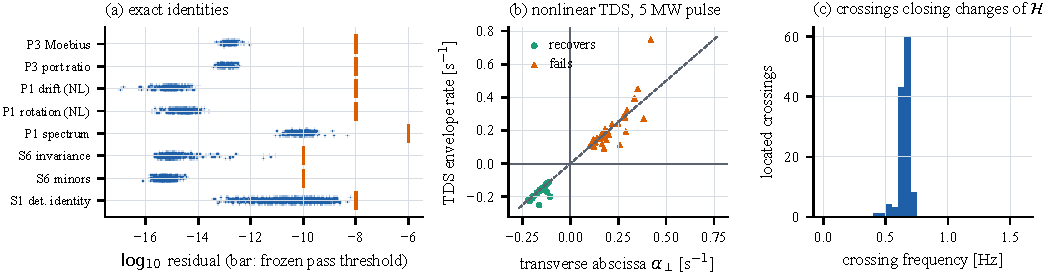
\includegraphics[width=\textwidth]{fig_mc.pdf}
\caption{Monte Carlo validation. (a)~Residuals of the exact identities (S1,
S6 synthetic; P1, P3 IEEE-39) against their frozen thresholds (bars).
(b)~Nonlinear TDS envelope growth rate versus the transverse abscissa for 80
random IEEE-39 policies and portfolios (dashed: identity). (c)~Frequencies of
the transverse eigenvalues that close the 120 changes of $\Hy$ on random policy
paths (post-hoc re-bisection; Table~\ref{tab:mc}, note c).}
\label{fig:mc}
\end{figure*}

\emph{Deviations from the preregistration.}
\begin{enumerate}
\item The P1 spectral-identity rule matched the numerically split Jordan pair
($\mathcal{O}(\sqrt{\epsilon\|A\|\omega_B})\approx10^{-5}$). It was amended
before the run, with the threshold unchanged.
\item The P2 rule failed as implemented (above).
\item In S7, three coalescence-class draws contained a genuine zero crossing.
In addition, 183 draws were left undecided by the device-flip rule, because
synthetic device blocks are not block diagonal; no Kundur holdout bracket was
undecided.
\item Two P1 draws needed a redrawn off-equilibrium state that stayed inside
the algebraic chart.
\end{enumerate}

% =========================================================================
\section{Scope Checks and Limitations}\label{sec:limits}

\subsection{Nonlinear finite disturbances: a negative result}\label{sec:nonlinear}
Nonlinear composability is a scope check, not a contribution. Three frozen
disturbance families were used: a bus-16 load pulse (D1), an SG36
mechanical-power dip (D2), and a GFL output dip (D3). Model-scope guards were
declared beforehand (Appendix~\ref{app:tds}). Inside these guards, the
finite-disturbance hypergraph equals the spectral $\Hy(\theta)$ in every tested
case (six point-family combinations; Fig.~\ref{fig:nonlinear}). No
transversely stable portfolio fails inside the guards: 84 of 96 thresholds are
guard activations (GFL voltage band, stabilizer limit). Earlier preregistered
runs confirmed all 32 declared small-disturbance verdicts, and P4 extends this
to 80 random cases. The three examined oscillatory boundaries are subcritical
Hopf points \cite{kuznetsov2004bifurcation}, with first Lyapunov coefficients
$+0.0095$, $+0.025$, and $+0.026$. Beyond the guards the model does not decide.

\begin{figure*}[!t]
\centering
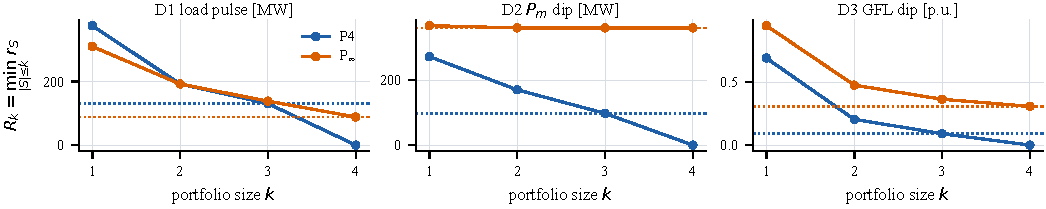
\includegraphics[width=\textwidth]{fig_nonlinear.pdf}
\caption{Finite-disturbance resilience radii $R_k=\min_{|S|\le k}r_S$ of the
IEEE-39 core at P4 and P$_\infty$ (TDS, phasor DAE). Dotted: model-scope radius
$\rho_{\rm scope}$. Below it the nonlinear hypergraph equals $\Hy(\theta)$;
above it every threshold is a guard activation.}
\label{fig:nonlinear}
\end{figure*}

\subsection{Limitations}
\begin{itemize}
\item \emph{Model.} The model is a phasor DAE, not an electromagnetic transient
model. It has no converter current limits, ride-through logic, or DC link, and
the IEEEX1 exciter is harmonized. The frozen models have no primary frequency
restoration, so all stability statements are transverse. The documented
governors change the P4 conclusion (Table~\ref{tab:gov}).
\item \emph{Independent implementation.} ANDES reproduces the power flow, the
base inter-area mode (within 4.1\%), and the governor damping direction. It
does not implement the converter model, so no portfolio result is claimed as
independently reproduced.
\item \emph{System dependence.} On the documented IEEE 68-bus system
\cite{canizares2015benchmark}, which is reproduced to 15/15 modes within
$5\times10^{-4}$~Hz, the preregistered four-candidate policy map is empty.
Policy dependence appears only at $\ge6$ of 12 replaced plants. On the Kundur
system, 61/61 and 36/36 policy lines change $\Hy$.
\item \emph{Mechanism scope.} No rank, path, or cycle explanation is claimed
(Section~\ref{sec:ieee39}-C). The Neumann walk expansion is non-executable in
the relevant band.
\item \emph{Numerics.} Labels are numerically exact, not interval-certified,
and 1.5\% of policy-map points are unresolved. No stability certificate is
claimed: sampled small-gain screens give $\rho=2.9$--$12.3>1$, and a local
Lyapunov bound reaches $\le10^{-11}$ of the measured threshold.
\item \emph{Scalability.} Enumerating $2^m$ labels is exponential, and
minimum-cardinality destabilization is NP-hard. Equation~\eqref{eq:fact1}
evaluates every portfolio from one base network and $m$ local increments, but
it does not remove the combinatorics.
\end{itemize}

% =========================================================================
\section{Discussion}\label{sec:discussion}
Table~\ref{tab:methods} places the work among established method families.
The hypergraph does not replace any of them, and its per-portfolio labels
\emph{are} generalized Nyquist tests. What is added is the organization of those
labels over binary replacement decisions, their network-closure anatomy, and
their movement with the converter policy. Flagship-only Nyquist, single-port
impedance, and short-circuit-ratio screens miss the coalition changes on
IEEE-39. Modal-sensitivity, additive, and pairwise predictors of the four-unit
instability were correct in 22, 30, and 38 of 52 cases, respectively.

\begin{table}[!t]
\centering
\caption{Relation to established method families}\label{tab:methods}
\setlength{\tabcolsep}{2.5pt}
\footnotesize
\begin{tabular}{@{}L{0.30\columnwidth}L{0.64\columnwidth}@{}}
\toprule
Family & Relation to this work \\
\midrule
Generalized Nyquist \cite{macfarlane1977gnc} & per-portfolio test; our labels are GN tests \\
Impedance / SCR \cite{sun2011impedance, xin2016gscr} & configuration screens; miss coalition changes \\
Small gain, passivity & sampled small-gain screen fails ($\rho=2.9$--$12.3$) \\
$\mu$ / robust stability \cite{poljak1993robust} & NP-hard in general; no priority claimed \\
Sparse stability radius \cite{katewa2020sparse} & continuous perturbations, not binary replacement \\
$N\!-\!k$ minimal sets \cite{bienstock2010nk} & static analogue; ours is dynamic, transverse, and policy dependent, with network-closure anatomy \\
Selective modal analysis \cite{perezarriaga1982sma} & explains modes; does not enumerate coalitions \\
Continuation / Hopf \cite{kuznetsov2004bifurcation} & boundaries are subcritical Hopf points \\
Energy / Lyapunov & local bound $\le10^{-11}$ of the threshold \\
Higher-order modal \cite{sanchezgasca2005higher} & requires $f_zD^2\psi$ (Appendix~\ref{app:curv}) \\
\bottomrule
\end{tabular}
\end{table}

% =========================================================================
\section{Conclusion}
The minimal incompatibility hypergraph $\Hy(\theta)$ is defined exactly in
transverse coordinates, changes only at imaginary-axis crossings, and
characterizes the portfolios that are safe in every implementation order (C1).
Its non-additivity is the principal-minor hierarchy produced by network
closure of local, affine replacement actions. At each of ten frozen IEEE-39
boundaries, no truncation below the cardinality of the changing minimal
coalition reaches the characteristic zero (C2). The port derivative gives
exact boundary normals and iterative retuning, and symmetry deflation extends
the test to zero-frequency crossings (C3).

The reactive policy reorganizes the structure. The specific four-unit witness
is conditional on the absence of primary frequency control, while policy
dependence persists with documented governors. Within model scope, nonlinear
simulation reproduces $\Hy$ exactly. Neither interaction rank nor network paths
explain the witness order. Every statement was tested by preregistered Monte
Carlo suites; one rule failed as implemented and is disclosed with its
separate post-hoc correction. Limiter-equipped, governed, and mixed grid-forming
benchmarks require new, separately versioned models.

\appendices
\section{Proof Details}\label{app:proofs}
\emph{Nonlinear identities in Theorem~\ref{thm:transverse}.} Fix $x$ in the
chart domain, let $z=\psi(x)$, and set $x_c=x+c\,w$. Speeds enter the reduced
equations only through $\dot\delta=\omega_B(\omega-1)$ and, for a GFL, through
$\dot\vartheta=k_{p,\rm pll}v_q+x_{\rm pll}$. In both, the shift adds the
constant $c\,\omega_B$ to the angle derivatives and nothing else. The
power-form swing equation with $D=0$ does not contain $\omega$ on its
right-hand side, the stabilizer uses electrical power, and the network is
frequency independent. Hence $\psi(x_c)=\psi(x)$ and
$r(x_c)=r(x)+c\,\omega_BR_x$. The rotation identity follows from
$\psi(x+\phi R_x)=e^{j\phi}\psi(x)$ and the invariance of $f$ under a common
rotation of angles and voltages.

\emph{Locality in Theorem~\ref{thm:factorization}.} On the common realization
$f_x$ is block diagonal by device. $f_z$ and $g_x$ couple a device only to the
two channels of its own bus, and the device contribution to $g_z$ is a
$2\times2$ block on that bus. Hence
$g_x(sI-f_x)^{-1}f_z=\sum_{\rm devices}E_bG_b(s)E_b^\top$, where $G_b$ is the
device's $2\times2$ admittance. With network and load terms common to all
vertices, $T_S-T_0=\sum_{i\in S}E_i\Delta Y_iE_i^\top$. $\Delta Y_i$ does not
depend on $S$ because every device stays at its common intensive equilibrium.
On the direct (non-common) path the locality residual is bounded by the
power-flow tolerance and was measured below $8\times10^{-8}$.

\emph{Corollary~\ref{cor:closure}.} If member $i$ alone has no eigenvalue at
$s^*$, then $\det(I+M_{ii})=\det T_{\{i\}}(s^*)/\det T_0(s^*)\neq0$, so the
zero of \eqref{eq:fact2} is a zero of $\det(I+Q_{SS})$. With $K_o=0$,
$\det(I+Q_{SS})=1$.

\section{Second-Order Curvature Audit (Supporting Methodology)}\label{app:curv}
On the same DAE, three reduced models of the response to a bus-16 load pulse
were compared with the full nonlinear solution (Fig.~\ref{fig:curvature}):
\begin{itemize}
\item linear;
\item complete second order;
\item second order without the algebraic curvature $f_zD^2\psi$.
\end{itemize}
At 2~MW the complete second-order model is 170--450 times more accurate than
the linear one in frequency and 750--3400 times in bus voltage (slope 3.0--3.2).
Dropping $f_zD^2\psi$ breaks the rotation/drift symmetry at second order and
makes the frequency prediction 570--1700 times worse than linear. With the
center-subspace component removed, the device curvature alone is still no
better than linear. This is a consistency requirement of second-order reduction
\cite{sanchezgasca2005higher}, not a novelty.

\begin{figure}[!t]
\centering
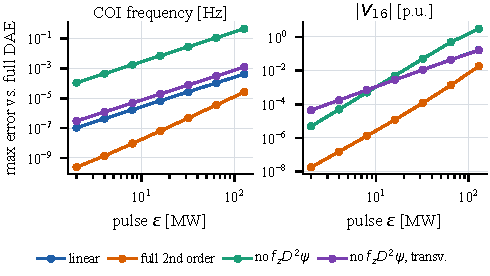
\includegraphics[width=\columnwidth]{fig_curvature.pdf}
\caption{Second-order reduced response of the triple 30+33+35 at P4 against the
full DAE. The complete second-order model requires $f_zD^2\psi$.}
\label{fig:curvature}
\end{figure}

\section{Monte Carlo Constructions}\label{app:mc}
\emph{S1.} $n\sim U\{8,\dots,40\}$. The transverse spectrum has real parts in
$[-2,1]$ (with $|\mathrm{Re}|\ge0.01$) and imaginary parts in $[0.5,10]$. Odd
draws plant one real eigenvalue at $\pm u$, with $u$ log-uniform in
$[10^{-5},5\times10^{-4}]$. $P=Q(I+0.3G)$ with $Q$ Haar orthogonal.
\emph{S2.} $A(\delta)=A_0+\sum\delta_iA_i$ with $m\in\{4,5,6\}$, $n=10$,
$\alpha(A_0)\in[-1,-0.2]$, and rank-2 actions; lattice search is exhaustive.
\emph{S3.} Actions $A_i+pB_i$ on a 401-point grid; 50-step bisection.
\emph{S4.} $B(S)=B_0+\sum_{i\in S}N_i$, $B_0$ Metzler, $N_i\ge0$, under random
similarity ($\mathrm{cond}\le10^3$); the control uses random signs.
\emph{S5.} $G(n,p)$ with $n\in[7,10]$, $p\in[0.3,0.8]$, $k\in\{3,4,5\}$.
\emph{S6.} Complex Gaussian $M$ with 3--5 blocks of size 2 and random block
basis changes.
\emph{S7.} Random descriptors ($n_x\in[10,30]$, $n_z\in[6,20]$,
$f_x=A+f_zg_z^{-1}g_x$) with five event classes. The relocation uses
$\beta=\beta_2=1$ and the consistency pair $(2,0.5)$.
\emph{P1--P4.} Direct-path solutions (full AC equilibrium, central-difference
Jacobians); P3 uses the common realization of Lemma~\ref{lem:affine}. Seeds and
rules are fixed in the preregistration file.

\section{Nonlinear Simulation Definitions}\label{app:tds}
The TDS integrates the full DAE (BDF, relative tolerance $10^{-7}$, maximum
step 0.05~s), with Newton network solutions at every step. A 0.5-s disturbance
is followed by 30~s of free response. $D(t)$ is the larger of the transverse
state and voltage deviations, normalized by $10^{-3}$ and $10^{-2}$.
\begin{itemize}
\item \emph{Recovers:} $D$ decays below 10\% of its early peak with a negative
envelope rate.
\item \emph{Fails:} $D$ exceeds twice the early peak with positive growth over
the last 10~s, or the relative rotor angle exceeds $\pi$.
\item \emph{Outside model scope:} a guard trips. The guards are bus voltage in
$[0.8,1.2]$; GFL terminal voltage in $[0.9,1.1]$; GFL current or apparent power
$\le1.2$; reactive power $\le1.0$; PLL or speed frequency in $[-3,1.8]$~Hz; COI
frequency within $\pm0.5$~Hz; field voltage within the documented exciter
limits; and stabilizer output $\le0.1$ (per unit on the device base).
\end{itemize}
Thresholds $r_S$ come from continuation on a frozen amplitude grid followed by
bisection. The minimum of the scope-censored thresholds defines
$\rho_{\rm scope}$.

\section*{Reproducibility}
The final scientific evidence state is frozen at commit \texttt{b9f274e2}.
The post-freeze evidence addenda cited here are \texttt{f775db89} (boundary
anatomy), \texttt{7a772808}/\texttt{f2946257} (Monte Carlo preregistration and
amendment), and \texttt{cfe9fe4b} (Monte Carlo results). Code, frozen
configurations, and the source data of every figure are available from the
author and in the project repository.

\balance
\bibliographystyle{IEEEtran}
\bibliography{references}

\end{document}
